\section{Algorismes i Implementacions}
Existeixen diverses implementacions dels recollidors de memòria brossa per diferents casos d'ùs; totes les implementacions segueixen el mateix algoritme base: 

\subsection{Algoritme Bàsic}
Totes les implementacions \textbf{marquen} les regions de memòria candidates a ser eliminades i les \textbf{eliminen}.

Per definir els objectes que es poden marcar, definim els següents estats dels objectes:

\begin{figure}[h]
    \centering
    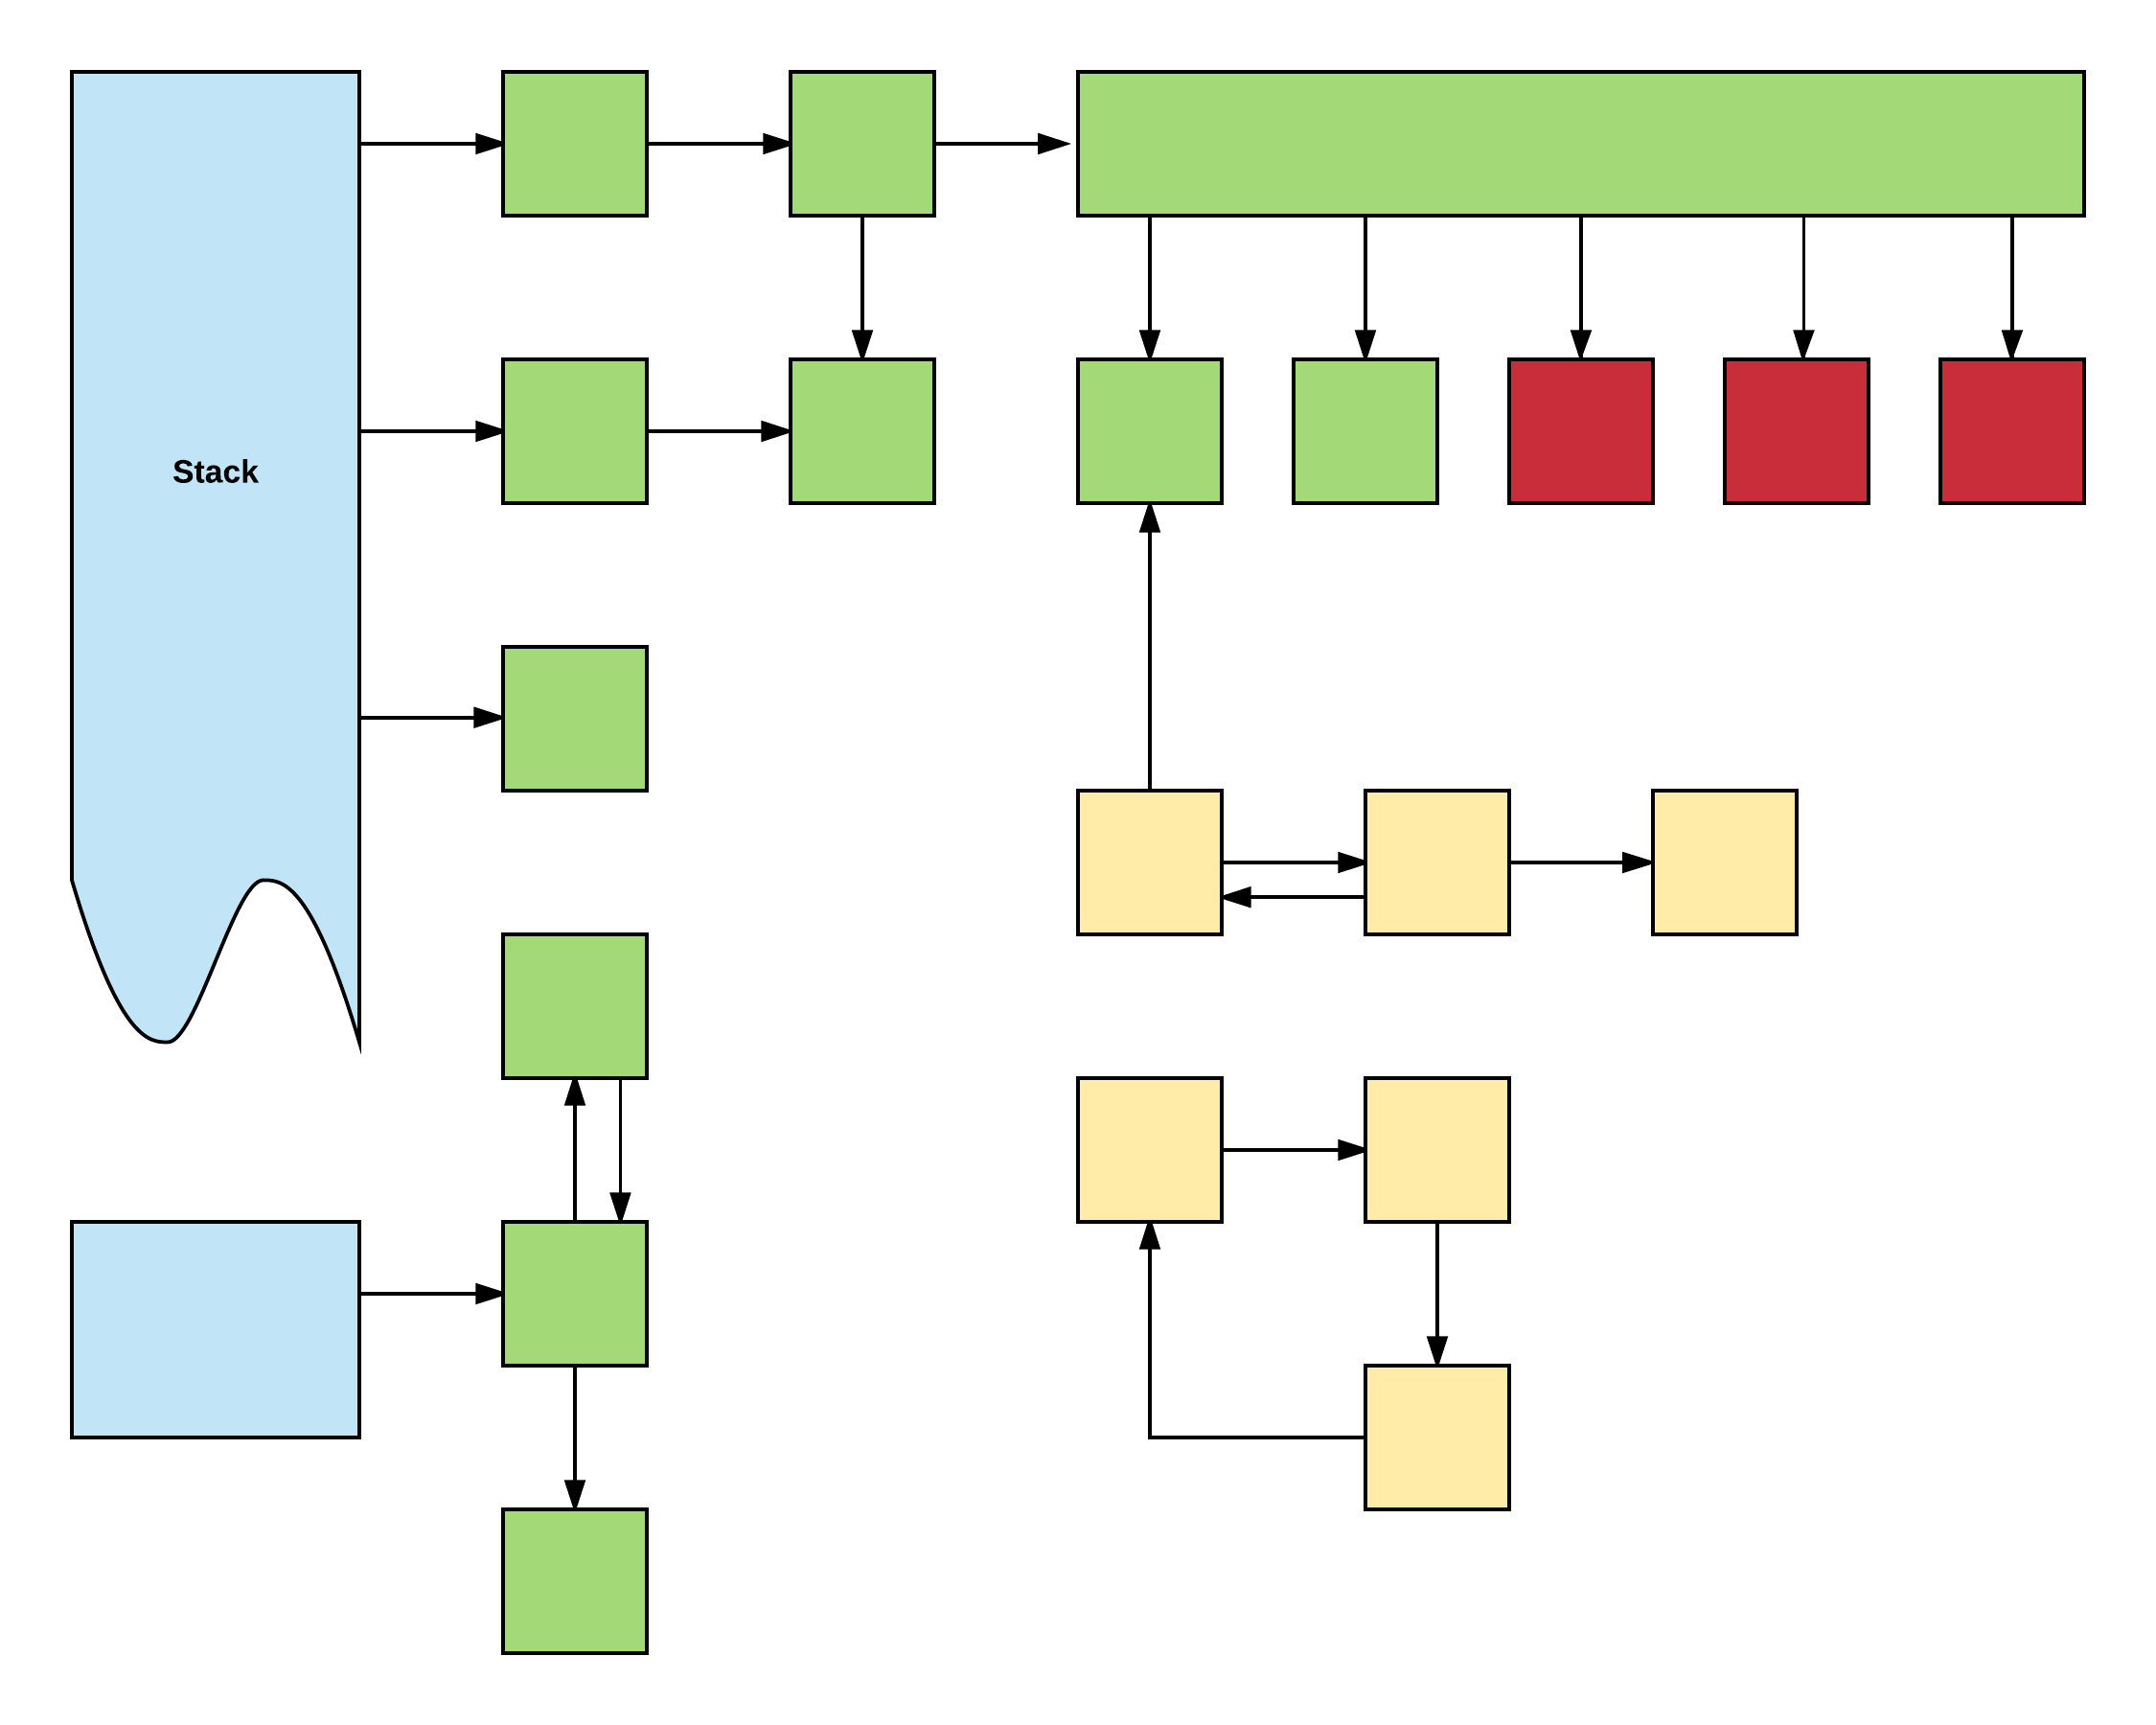
\includegraphics[width=\textwidth, height=8cm]{memory-objects-example.png}
    \caption{Exemple d'un estat dels objectes en un programa.}
\end{figure}

Al exemple, extret de blog \textit{The danger of garbage-collected languages}\cite{gbProblems}, tenim objectes 'vius' pintats de verd, objectes 'morts' pintats de groc i objectes que no es faran servir més pintats de vermell.

Els objectes morts (no tenen cap referència) són els que els algoritmes de GC marquen com a triats. D'altra banda, els objectes que no es faran servir més no poden ser marcats, ja que segueixen sent referenciats.

Un cop marcats els objectes, el següent pas és eliminar els objectes (o regions de memòria). Existeixen dues estratègies:

\begin{itemize}
    \item Esborrar : S'esborren els objectes i l'assignador de memòria mantè una llista d'espais lliures.
    \item Esborrar + Compactar: S'esborren els objectes i es compacten a memòria, l'assignador de memòria només manté l'inici de l'espai lliure.
\end{itemize}


\subsection{Implementacions a Java}

Java té diverses implementacions de GC, per diferents casos d'ús. Totes elles divideixen el heap de la JVM\footnote{La Java virtual machine és l'entorn d'execucció de programes Java} en generacions:

\begin{enumerate}
    \item Generació jove: Lloc on s'assignen els nous objectes. Tots els nous objectes es crean en la regió \textit{eden}, dins de la generació jove. 
    \item Generació de supervivents: Dues regions on els objectes de l'eden no eliminats són guardats. Els objectes guanyen 'edad' al avançar entre regions supervivents. Es troba dins de la generació jove.
    \item Generació antiga: Regió on es guarden els objectes supervivents de GC.
    \item Generació permanent: Metadata de la JVM per tota l'execucció del programa
\end{enumerate}
\begin{minipage}{\textwidth}    %mantener en la misma pagina
Existeixen diferents GC depenen quina regió del heap s'omple:
\begin{itemize}
    \item \textit{Minor} garbage collection: Un cop s'ha omplert l'\textit{eden} es donen les següents accions:
    \begin{enumerate}
        \item Els objectes que no estan referenciats s'eliminen.
        \item Els altres es mouen a la regió de supervivents, amb edad = 1.
        \item Els objectes supervivents promocionen a generació antiga (donada una certa edad).
        \item Els objectes de la regió de supervivents augmenten en 1 la seva edad (o s'eliminen si no están referenciats).
    \end{enumerate}
    \item \textit{Major} garbage collector: Un cop la generació antiga està plena, involucra a tots els objectes del programa.
\end{itemize}
\end{minipage}

Sobre aquesta distribucció del heap, tenim les següents versions de GC:
\begin{itemize}
    \item Serial GC: Recol·lector senzill que funciona amb un únic thread per les recol·lecions \textit{minor} i \textit{major}. Utilitza el mètode d'esborrar i compactar; també ordena les regions de supervivents al principi del \textit{heap} per afavorir l'assignació de nous objectes.
    \item Parallel GC: Recol·lector que utilitza múltiples threads per gestionar l'espai al Heap. Existeixen dos opcions:
    \begin{itemize}
        \item Versió A: \textit{Multi-threading} per \textit{minor GC} i \textit{single-threading} per \textit{major} GC.
        \item Versió B: En les dues GC, s'utilitza \textit{multi-threading}.
    \end{itemize}
    \item Concurrent Mark Sweep (CMS): El procès de GC funciona concurrentment amb l'execucció del programa, per les \textit{major} GC. Dóna lloc a poques pauses d'execucció del programa\footnote{Els procesos de major i minor GC detenen tot el flux del programa, anomenat Stop the World Event al àmbit de Java}.
\end{itemize}

Cal destacar una última versió de GC implementada a Java (desde el JDK7), anomenada G1. Aquesta implementació no segueix les generacions/regions del heap exposades anteriorment. 

El G1 \textit{Garbage collector} divideix el heap en regions d'igual tamany, per marcar de forma concurrent i paral·lela els objectes. Un cop marcats els objectes dins les regions, el G1 comença a alliberar espai en les regions que es consideren més lliures. Aquesta versió té molt més rendiment que el CMS. 

Els casos d'ús de cada recol·lector recauen sobre el temps que s'inverteix en executar l'algoritme de GC, si la nostra aplicació busca rendiment s'haura de triar el CMS o G1.
